\documentclass[10pt]{article}
\usepackage{amsmath}
\usepackage{amsfonts}
\usepackage{amssymb}
\usepackage{verbatim}
\usepackage{courier}
\usepackage{graphicx}
\usepackage{subfig}
\usepackage{hyperref}
\usepackage{url}

\author{Joshua Horswill}
\title{ILL internship report}

\begin{document}
\maketitle
\tableofcontents
\newpage
\section{Introduction}
The aim of this project is to create a driver to compute the magneto-electric coupling of a multiferroic system. Multiferroic materials are defined by the possession of a coupling between at least two ferroic orders. The foci of this report are the calculations for materials that exhibit couplings between electric and magnetic properties. Specifically it would demonstrate a net magnetic moment, an intrinsic polarisation and a linear magneto-electric coupling. This is a type II multiferroic system, type I being a material whose transitions from paraelectric and ferroelectric states are distinct from magnetic transitions \cite{Hur2004}\cite{goto2004ferroelectricity}.

In order to determine this linear magneto-electric coupling for the type II material experimentally, the associated tensor $\bar{\bar{\alpha}}$ must be measured. This tensor can be described as the response of the polarisation of a system as a function of the applied magnetic field. It can simultaneously be described as the response of the magnetic order parameter as a function of the applied electric field (this parameter is given by $\vec{M} = \sum_j \vec{\mu}_j$ or for an antiferromagnetic material, $\vec{M} = \sum_j (-1)^j \vec{\mu}_j$) where $\vec{\mu}_j$ is the magnetic moment for the jth electron. These responses are of course linear.

The driver processes inputs and outputs of the various ab-initio functions (discussed later) so that it can generate the computation of this tensor $\bar{\bar{\alpha}}$ from a simulation of the electronic structure.

\section{Relation of the $\bar{\bar{\alpha}}$ tensor to the exchange integral $J$}

Lev Landau introduced a physical theory that attempted to create a general model of continuous and therefore second-order phase transitions. It is versatile in that it can be used in systems that are subject to external fields. Landau proposed that the free energy of any system should be analytic (continuous and therefore differentiable), and obey the same symmetry of the Hamiltonian. This allows the generation of a phenomenological expression for the free energy as a Taylor expansion in the order parameters - electric field and magnetic field \cite{landau1936theory}.

Using this theory it is possible to write an expression for $\bar{\bar{\alpha}}$ in terms of the second derivative of the free energy with respect to the electric and magnetic fields ($\vec{\mathcal{E}}$ and $\vec{\mathcal{H}}$ respectively):

\begin{equation*}
\bar{\bar{\alpha}} = -\frac{\partial^2 \mathcal{F}}{\partial \vec{\mathcal{E}}\partial\vec{\mathcal{H}}}\biggr\vert_{\vec{\mathcal{E}}=\vec{0}, \vec{\mathcal{H}} = \vec{0}}
\end{equation*}

For multiferroic systems, low-energy excitations are of a magnetic nature due to the material being a magnetic insulator. This means it is possible to describe this property by implementing an effective Hamiltonian that only takes into account the magnetic degrees of freedom. One of the models that fits these requirements particularly well is the Heisenberg Hamiltonian. For example, let us suppose that a system can be described by this Hamiltonian for the Fermi level (magnetic) properties:

\begin{equation}
\hat{H} = E_0 - \sum_{\langle i,j \rangle} J_{i,j}\hat{\vec{S_i}}\cdot \hat{\vec{S_j}}
\end{equation}

where $E_0$ is the energy associated with all non-magnetic degrees of freedom and $\langle i,j \rangle$ represents nearest neighbour exchanges (since the interaction is local), $J_{i,j}$ is the magnetic exchange integral between atoms i and j, with atomic spin $\hat{\vec{S_i}}$ and $\hat{\vec{S_j}}$ respectively. By observing the polar magnetic phase in which the magneto-electric coupling occurs, it is possible to write a statistical mechanical equation of state for the free energy ($\mathcal{F} = U - TS$ where U is internal energy, T is temperature and S is entropy):

\begin{equation*}
\mathcal{F} = E_0 - \sum_{\langle i,j \rangle} J_{i,j}\langle \hat{\vec{S_i}}\cdot \hat{\vec{S_j}} \rangle - \sum_{i}g\mu_{B}\langle \vec{S_i}\rangle \cdot \mathcal{\vec{H}} - \vec{P}\cdot \mathcal{\vec{E}} - TS
\end{equation*}

where $\langle \rangle$ denotes the thermal average of the quantity and $J_{i,j}$ represents the effective magnetic integrals between the ith and jth magnetic ions. 

It is known that the thermal probability of a state being occupied, in an energetically gapped system such as this, is varying very quickly as soon as the temperature $T$ is slightly larger or smaller than the critical temperature of the transition ($T_c$). In the paramagnetic phase ($T > T_c$, where for all magnetic states, thermal energy $k_B T \gg E_I - E_0$, where $E_I$ is the energy of the Ith magnetic state) all eigenstates have an equivalent probability $P(E = E_I) = \exp(-\beta E_I)/Z \simeq 1/N$ where N is the number of magnetic eigenstates and Z is the partition function for the system. 

Consequently, the free energy $\mathcal{F}$ is dominated by the entropy term. However, in the phase where the system is magnetically ordered ($T < T_c$), the probability $P(E = E_{ground})$ dominates so that $\mathcal{F}$ is dominated not by entropy but by the energetic term $U$. Now we can neglect the entropy contribution in the calculation of $\bar{\bar{\alpha}}$ as soon as the temperature is slightly smaller than $T_c$.

To first order, $\bar{\bar{\alpha}}$ can resultantly be written as:

\begin{equation}
	\bar{\bar{\alpha}} = \sum_{\langle i,j \rangle} \frac{\partial J_{i,j}}{\partial \vec{\mathcal{E}}}\biggr\vert_{\vec{\mathcal{E}}=\vec{0}}\otimes\biggr(\frac{\partial \langle \vec{S_i}\rangle}{\partial \vec{\mathcal{H}}}\biggr\vert_{\vec{\mathcal{H}} = \vec{0}}\cdot\langle\vec{S_j}\rangle + \langle\vec{S_i}\rangle\cdot\frac{\partial \langle \vec{S_j}\rangle}{\partial\vec{\mathcal{H}}}\biggr\vert_{\vec{\mathcal{H}}=\vec{0}}\biggr)
\end{equation}

This means that the derivative of the exchange integrals with respect to the electric field and the derivative of the local magnetic moments with respect to the magnetic field will need to be calculated. The former will require accurate ab-initio evaluation of the $J_{i,j}$ integrals and the latter can be obtained using standard spin wave calculations (see \cite{anderson1951limits,kubo1952spin,oguchi1960theory}). In section 3 we will discuss the details of how these goals will be achieved.

\section{Computing the magnetic exchange term from nuclei displacement}

Iniguez argues that the lattice-mediated part of the linear magnetoelectric response of magnetic insulators is dominant in materials displaying strong magnetoelectric couplings \cite{iniguez2008first}. These insulators allow control of their magnetic properties through the manipulation of an external electric field. The magnetization induced by the application of an electric field is given by:

\begin{equation*}
\mathcal{M}_j(\mathcal{E}) = \sum_i \bar{\bar{\alpha_{ij}}}\mathcal{E}_i
\end{equation*}

Where $\alpha$ is the linear magnetoelectric tensor, i and j label spatial directions and $\mathcal{E}$ is the electric field. The magnitude of this response is limited by the magnetic and dielectric susceptibilities as $\alpha^2_{ij} < \chi^m_{jj}\chi^d_{ii}$, suggesting that strong ME coupling occur in materials that demonstrate large dielectric and magnetic responses. This means that large magnetoelectric effects will correlate to significant electronic hybridizations or orbital rearrangements induced by applied electric fields. This is caused by a magnetic response via spin-orbit or exchange-strictive effects. Strong dielectric responses are never purely electric - they are driven by the structural changes induced by the applied field. We can deduce that large ME effects will be based on lattice-mediated mechanisms in systems where the spin-orbit coupling is relatively large. 

The associated magnetoelectric coupling is computed from the first derivative of the exchange integral $J$ as a function of an applied electric field $\mathcal{E}$, as seen in equation (2). The main effect of an electric field on an ionic insulator is to displace the ions (nuclei). This displacement can be computed from:
\begin{itemize}
	\item The Hessian matrix of the
	energy $\mathcal{H} = \frac{\partial^2 E}{\partial \mathbf{d} ^2} $ obtained
	from a mean-field DFT calculation (see section 4 for details)
	\item The Born dynamical effective charges $q^*$ which corresponds to the second
	derivative of the energy with respect to the field and displacement
	\item Newton's 2nd law
\end{itemize}

\begin{equation}
	q^* \mathcal{E} = -\mathcal{H} d
\end{equation}

which implies that the displacement induced by an electric field is equivalent to:

$$ d = -\mathcal{H}^{-1} q^* \mathcal{E} $$

This equation also suggests that the main response of a ferroelectric compound to an applied electric field will be a geometry modification that can be evaluated by the displacement of the system ions from their equilibrium position. 

We can evaluate the Hessian and the Born charges with DFT calculations as they both depend on the whole electron density functionals. The correlation interactions among the Fermi electrons will have only negligible effects on these quantities, and so it is safe to use DFT approximations with the suitable functionals.

In summary our approach is as follows:

\begin{enumerate}
	\item Optimise the structure's geometry to minimise the total energy of the system using DFT
	\item From this, obtain the associated optimal Hessian matrix and Born tensor
	\item Solve the resultant linear system of equations in equation (3) for charge displacement
	\item For a range of displacements calculate the magnetic exchange integral $J$ using an embedded fragment, wavefunction-correlated method since DFT cannot generate accurate calculations for this part. This involves the consideration of many Slater's determinants: the evaluation of many antisymmetric superposition of states that each represent a given system configuration. This is required because the properties of J (governed by the Fermi level electrons) rely on a strongly-correlated, configuration-sensitive system. An example of this would be the SAS+S method (see section 5 for more details). This allows us to generate $\frac{\partial J}{\partial d}$
	\item Computing displacement for a range of $\mathcal{E}$ allows for the generation of $\frac{\partial d}{\partial E}$, and therefore the numerical evaluation of the derivative of the spin Hamiltonian parameters as a function of the applied electric field:
	\begin{equation*}
	\dfrac{\partial J}{\partial \mathcal{E}} = \dfrac{\partial J}{\partial d}\dfrac{\partial d}{\partial \mathcal{E}}
	\end{equation*}
	\item Use non ab-initio spin wave methods to determine $\frac{\partial\langle S_{i,j}\rangle}{\partial H}$ and $\langle S_{i,j}\rangle$
	\item Obtain $\bar{\bar{\alpha}}$
\end{enumerate}

This method has successfully been applied to YMnO$_3$ using SAS+S to calculate the exchange integral for each value of the displacement, since it was designed specifically for the purpose of precise evaluation of magnetic excitations \cite{varignon2013ab}. The configuration interactions for ligand-to-metal charge transfers and screening effects were included explicitly, and so appropriate embedded fragments were implemented. It was shown that when the electric field was applied perpendicular to the MnO$_3$ planes, $\frac{\partial J}{\partial \mathcal{E}}$  was negligible in value. When the electric field was applied in-plane, the absolute value of J increases when the field is parallel to the Mn-Mn bond. However, the spin-orbit coupling plays a negligible role in the ME response, which suggests there is be a different mechanism that is responsible.

\subsection{The Simulation Environment}
The embedded fragments are designed to include the configuration states that describe the prioritised physical processes. It has been argued that in wide-gap magnetic insulators, $J$ is determined from strongly local electronic interactions involving two magnetic centers \cite{de1999local}. These fragments were embedded in an environment reproducing the main effects as the rest of the crystal, as discussed towards the end of section 5.1. To achieve this we must include the Pauli exclusion effects of surrounding electrons and the influence of a non-local Madelung potential (nuclei-electron interactions simplified through ions being approximated as a set of point charges). The exclusion effect can be modelled through a surrounding total ionic pseudopotential (TIP, see \cite{winter1987theoretical} for example usage of this method). The Madelung potential can be recreated through an array of renormalised point charges assigned to atomic positions \cite{gelle2008fast}.

\section{Density Functional Theory (DFT)}
\subsection{Many-Body Schrödinger equation}
The nonrelativistic time-dependent Schrödinger equation for an individual particle is given by:

\begin{equation}
	\biggr[-\frac{\hbar^2}{2m}\nabla^2+\mathcal{U}(\textbf{r},t)\biggr]\Psi(\textbf{r},t) = i\hbar\frac{\partial}{\partial t}\Psi(\textbf{r},t)
\end{equation}

where $\mathcal{U}(\textbf{r},t)$ is the external potential and $\Psi(\textbf{r},t)$ is the wavefunction of the particle being described. This can be generalised to a system of $N$ electrons, the positions and mass of which are denoted by \textbf{$r_n$} and $m_e$ respectively, and $M$ nuclei, whose positions and mass are given by \textbf{$R_{I_n}$} and $m_{I_n}$ respectively. If we use atomic units ($\hbar = m_e = \frac{e^2}{4\pi\epsilon}$) we can expand the Schrödinger equation from equation (4) by adding the many-body terms:

\begin{gather*}
	\biggr(-\frac{1}{2}\biggr(\sum_n\nabla^2_{\textbf{r}_n}+\sum_{n}\frac{\nabla^2_{\textbf{R}_{I_n}}}{m_{I_n}}\biggr)+\frac{1}{2}\sum_{n\not=m}\frac{1}{|\textbf{r}_n-\textbf{r}_m|}-\sum_{n,m}\frac{Z_{I_m}}{|\textbf{r}_n - \textbf{R}_{I_m}|}\\
	+\frac{1}{2}\sum_{n\not=m}\frac{Z_{I_n}Z_{I_m}}{|\textbf{R}_{I_n}-\textbf{R}_{I_m}|}\biggr)\Psi = i\frac{\partial\Psi}{\partial t}
\end{gather*}

where the term $$\hat{T} = -\frac{1}{2}\biggr(\sum_n\nabla^2_{\textbf{r}_n}+\sum_{n}\frac{\nabla^2_{\textbf{R}_{I_n}}}{m_{I_n}}\biggr)$$ is the kinetic contribution and $$\hat{V}=\frac{1}{2}\sum_{n\not=m}\frac{1}{|\textbf{r}_n-\textbf{r}_m|}-\sum_{n,m}\frac{Z_{I_m}}{|\textbf{r}_n - \textbf{R}_{I_m}|}\\
+\frac{1}{2}\sum_{n\not=m}\frac{Z_{I_n}Z_{I_m}}{|\textbf{R}_{I_n}-\textbf{R}_{I_m}|}$$ is the potential contribution, taking into account interactions between electrons and other electrons, electrons and nuclei, and nuclei and other nuclei.  $i\frac{\partial}{\partial t}$ is the energy operator, giving energy eigenvalues from the total wavefunction.\\

For most systems this equation cannot be solved exactly and so we must include firstly the Born Oppenheimer approximation. This uses the fact that an electron is almost 2000 times less massive than the nucleus, and so the positions of the nuclei can be treated as fixed when trying to generate the electron wavefunction, and therefore the source of the Coulomb interaction is always static. The total electron wavefunction becomes separable, with an electronic part $\Psi_e$ and a nuclear part $\Psi_{nu}$ where $R_n$ are treated only as parameters:

\begin{equation*}
	\Psi_{electron}(\textbf{r}_n,\textbf{R}_n) =  \Psi_e(\textbf{r}_n;\textbf{R}_n)\Psi_{nu}(\textbf{r}_{n})
\end{equation*}

This allows us to generate two energy eigenvalue equations for each wavefunction and try to solve for $\Psi(\mathbf{r_1},\mathbf{r}_2,...\mathbf{r_n})$ \cite{rebolini2014range}. 

\subsection{Hartree-Fock Theory}
The Hartree-Fock method is the basis of molecular orbital theory, which postulates that in a material, each electron's motion can be described by a single-particle function that does not depend explicitly on the neighbouring electron's instantaneous motion. These orbitals are only approximations of reality however; the only exact eigenfunctions of the full electronic Hamiltonian are for hydrogen or He$^+$ where the system contains only one electron. However, as long as we consider these molecules near their geometrical energetic equilibrium (see step one of section 3), Hartree-Fock theory provides a good starting point for more detailed theoretical methods (e.g many-body perturbations, single-reference configuration interactions - see section 5). It is designed to solve the electronic Schrödinger equation resulting from the reduced time independent equation after using the Born-Oppenheimer approximation, as in section 4.1. It starts from `pretending' that in multiple-electron systems, electron-electron interactions can be ignored in order to render the Hamiltonian separable; the electronic wavefunction becomes a product of N orbitals, where N is the number of electrons being considered in the quantum system \cite{sherrill2000introduction}. This is called the Hartree product and can be written generally as:

\begin{equation}
	\Psi_{HP}(\mathbf{r}_1,\mathbf{r}_2,...,\mathbf{r}_N) = \phi_1(\mathbf{r}_1)\phi_2(\mathbf{r}_2)...\phi_N(\mathbf{r}_N)
\end{equation}

This fails to satisfy the fermionic antisymmetry principle i.e. the wavefunction should be antisymmetric when interchanging any set of spin-space coordinates ($x,y,z$ spatial and $\alpha$ spin where a space-spin vector is given by $\mathbf{x}=(\mathbf{r},\omega)$ where $\omega$ is the general spin coordinate for $\alpha$. We can also change our orbital notation from spatial $\phi(\mathbf{r})$ to spin orbital $\chi(\mathbf{x})$. The spin orbital is usually given by $\chi(\mathbf{x}) = \phi(\mathbf{r})\alpha(\omega)$. This turns equation (5) into:

\begin{equation*}
	\Psi_{HP}(\mathbf{x}_1,\mathbf{x}_2,...,\mathbf{x}_N) = \chi_1(\mathbf{x}_1)\chi_2(\mathbf{x}_2)...\chi_N(\mathbf{x}_N)
\end{equation*}

which is still not antisymmetric in general, as it requires

\begin{equation*}
	\chi_1(\mathbf{x}_2)\chi_2(\mathbf{x}_1) = -\chi_1(\mathbf{x_1})\chi_2(\mathbf{x_2})
\end{equation*}

This is where Slater determinants come in. For a two electron system we can write an antisymmetric spin orbital as $$\Psi(\mathbf{x}_1)\Psi(\mathbf{x}_2) = \frac{1}{\sqrt{2}}[\chi_1(\mathbf{x_1})\chi_2(\mathbf{x_2})-\chi_1(\mathbf{x}_2)\chi_2(\mathbf{x}_1)]$$

This can be written as a determinant:

\begin{equation*}
	\Psi(\mathbf{x}_1,\mathbf{x}_2) = \frac{1}{\sqrt{2}}
\begin{vmatrix}
	\chi_1(\mathbf{x}_1) & \chi_2(\mathbf{x}_2)\\
	\chi_1(\mathbf{x}_2) & \chi_2(\mathbf{x}_2) \\
	\end{vmatrix}
\end{equation*}

which can be generalised to:

\begin{equation}
	\Psi = \frac{1}{\sqrt{N}} =
	\begin{vmatrix}
	\chi_1(\mathbf{x}_1) & \chi_2(\mathbf{x}_1) & ... & \chi_N(\mathbf{x}_1) \\
	\chi_1(\mathbf{x}_2) & \chi_2(\mathbf{x}_2) & ... & \chi_N(\mathbf{x}_2) \\
	\vdots & \vdots &\ddots & \vdots \\
	\chi_1(\mathbf{x}_N) & \chi_2(\mathbf{x}_N) & ... & \chi_N(\mathbf{x}_N)
	\end{vmatrix}
\end{equation}

If you try to put two electrons in the same orbital i.e. set $\chi_1 = \chi_2$ then the wavefunction becomes zero. This is a mathematical form of Pauli's exclusion principle. If we have a list of the occupied orbitals we can shorten this form to ket notation, with the normalisation factor implied: $|ij...k\rangle$; see section 5. This way of writing electron wavefunctions assumes that electrons move independently of the others, and so Hartree-Fock theory is referred to as a `mean field' theory. 

Using this ket notation we can shorten the Hamiltonian to the following forms in order to bury some of the complexity in the evaluation of integrals. The singular-electron operator can be written as:

\begin{equation*}
	h(i) = -\frac{1}{2}\nabla_i^2-\sum_A\frac{Z_a}{r{iA}}
\end{equation*}

and the two electron operator can be written as:

\begin{equation*}
	v(i,j)=\frac{1}{r_{ij}}
\end{equation*}

so that the Hamiltonian becomes:

\begin{equation*}
	\hat{H}_{electron} = \sum_i h(i) + \sum_{i<j}v(i,j) + V_{NN}
\end{equation*}

where $V_{NN}$ is a constant for the fixed set of nuclear coordinates, so we can ignore if for now as this term only shifts the eigenvalues, with no effect on the eigenfunctions. Now we need to approach obtaining the molecular orbitals. If we are looking for a Hartree-Fock wavefunction in normalised Slater determinant form, and assert that the electronic energy is given by:

\begin{equation*}
	E_{electron} = \langle\Psi|\hat{H}_{electron}|\Psi\rangle
\end{equation*}

For symmetric energy expressions we can use something called the `variational theorem', which asserts that the energy is always an upper bound to the true energy. We can choose a `trial wavefunction' that depends on one or multiple parameters, and finding the parameter configuration that minimises the expectation value of the energy in the observed functional space. This allows for a better approximation of the system wavefunction. This is a key method in the the Hartree-Fock approach. In other words, $E_{electron}$ will be an overestimation of the true ground state energy unless $\Psi$ is equal to the exact ground state wavefunction of the system, but a tighter upper bound can be generated from tuning the trial wavefunction \cite{sakurai1994modern}. The energy-minimising orbital configuration can be obtained as a linear combination of the basis functions (Gaussian-type in LCAO) \cite{sherrill2000introduction}. 

We can rewrite the Hartree-Fock energy to achieve this purpose, by expressing it in terms of the integrals of one and two electron operators:

\begin{equation}
	E_{electron} = \sum_{i}\langle i|h|i\rangle + \frac{1}{2}\sum_{ij}[ii|jj]-[ij|ji]
\end{equation}

where

$$\sum_{i}\langle i|h|i\rangle = \int d\mathbf{x_1} \ \chi^*_i(\mathbf{x_1})h(\mathbf{r_1})\chi_j(\mathbf{x_1})$$

and

$$[ij|kl] = \int d\mathbf{x_1} d\mathbf{x_2} \ \chi^*_i(\mathbf{x_1})\chi_j(\mathbf{x_1})v(i,j)\chi^*_k(\mathbf{x_2})\chi_l(\mathbf{x_2})$$

which can be calculated using common existing computer algorithms.

\subsubsection{Hartree Fock Equations}
The assumption that the wavefunction can be approximated by a single Slater determinant of one spin orbital per electron is core to DFT. This single-reference space can be built upon by a perturbational model to achieve more accurate wavefunction solutions. The Hartree-Fock energy expression is by definition symmetric and so we know that the Slater determinant generating the lowest overall energy is the closest one can get to the true wavefunction in the assumed functional form. We must minimise the value of $E_{electron}$ from equation (7) with respect to the changes in the orbitals $\chi_i$. So far the orbitals $\chi$ have been assumed to be orthonormal, and so we must keep them that way through our variational procedure. This is done by employing `Lagrange's method of undetermined multipliers', where we use a Lagrangian $\mathcal{L}$ such
that:

\begin{equation*}
	\mathcal{L}[\{\chi_i\}] = E_{electron}[\{\chi_i\}]-\sum_{ij}\epsilon_{ij}(<i|j>- \ \delta_{ij})
\end{equation*}

where the coefficients $\epsilon_{ij}$ are undetermined Lagrange multipliers and the $<i|j>$ orbital inner product represents the overlap between the ith and jth spin orbitals. Setting the first variation of the Lagrangian equal to zero ($\delta\mathcal{L} = 0$) and doing some algebra we can generate the Hartree-Fock equations defining each orbital:

\begin{equation}
	h(\mathbf{x_1})\chi_i(\mathbf{x_1})+\sum_{j \not= i}\biggr(\int d\mathbf{x_2} \ |\chi_j(\mathbf{x_2})|^2r_{12}^{-1}\biggr)\chi_i(\mathbf{x_1})-\sum_{j \not= i}\biggr(\int d\mathbf{x_2} \ \chi_j^*(\mathbf{x_2})\chi_i(\mathbf{x_2})r_{12}^{-1}\biggr)\chi_j(\mathbf{x_1}) = \epsilon_i\chi_i(\mathbf{x_1})
\end{equation}

where $\epsilon_i$ is the energy eigenvalue corresponding to the ith orbital eigenfunction. This problem can be solved in two ways, the first being numerically, and the second solving it in a space spanned by the basis functions. Both solutions depend on the orbitals, and so we need to guess some initial orbitals and generate increasingly educated guesses iteratively. The first term in equation (8) represents the Coulomb interaction of an electron described by $\chi_i$ with the average charge distribution of the other electrons (mean field). 

\subsection{Hohenberg-Kohn theorems}

The electronic part of the Hamiltonian ($\hat{H}=\hat{T}+\hat{V}$) is the same for all N-electron systems after we assert the Born-Oppenheimer approximation. This means that the ground state wavefunction $|\Psi_0\rangle$ is completely determined by N and the electric interactions involving the nuclei. The ground state wavefunction for this Hamiltonian gives rise to a ground-state electronic density $n_o(\mathbf{r})$:

\begin{equation*}
	n_0(\mathbf{r})=\langle\Psi_0|\hat{n}|\Psi_0\rangle = \int\prod_{n=2}^{N}d\mathbf{r}_n|\Psi_0(\mathbf{r},\mathbf{r}_2,...\mathbf{r}_N)|^2
\end{equation*}

where $\hat{n}$ is the density operator. Therefore the ground state and associated density are both functionals of the number of electrons N and the ionic electrostatic potential. DFT, introduced by Hohenberg and Kohn in 1964, asserts two statements:

\begin{itemize}
	\item The ionic potential is determined uniquely by the ground-state electronic density functional, up to a constant.
	\item For all densities in an external potential (e.g the nucleic electrostatic potential) $n(\mathbf{r})$, their energy $E_V[n]\geq E_0$ ($E_0$ being the ground state energy), for N electrons in an external potential $V(\mathbf{r})$ \cite{haynes}. 
\end{itemize}

This means the issue of solving the Schrodinger equation for ground-states can be transformed into a variational problem of minimising the energy functional $E_V[n]$ with respect to the densities in an external potential $V_{ext}$ \cite{hohenberg1964inhomogeneous}. By writing the Hamiltonian in terms of the electronic operator and the external potential operator $\hat{H} = \hat{F}+\hat{V}_{ext}$ where: $$\hat{F} = -\frac{1}{2}\biggr(\sum_n\nabla^2_{\textbf{r}_n}-\sum_{n\not=m}\frac{1}{|\textbf{r}_n-\textbf{r}_m|}\biggr)$$

and defining the universal functional as:

$$F[n] = \min_{|\Psi\rangle\rightarrow n}\langle\Psi|\hat{F}|\Psi\rangle$$

We can define $E_V[n]$ as:
\begin{equation}
	E_v[n] = F[n]+\int d\mathbf{r} \ n(\mathbf{r})V_{ext}(\mathbf{r}) = \langle\Psi_n|(\hat{F}+\hat{V}_{ext})|\Psi_n\rangle
\end{equation}

Using the variational principle to obtain the inequality in statement (2) made in DFT \cite{haynes} we can assert that the ground-state density $n_0(\mathbf{r})$ minimises the functional $E_V[n]$, and the minimum value is the ground-state electronic energy $E_0$. Through this principle we can consider $N$-representable densities, the requirements of which are much weaker and satisfied by any well-behaved density. These are densities where the domain of the density is larger than the external potential. We do not know at face value if this density $n(\mathbf{r})$ arises from an antisymmetric N-body wavefunction, but it has been proven that any non-negative function can be written in terms of some $\Psi(\mathbf{r}_1,\mathbf{r}_2,...\mathbf{r}_n)$ \cite{gilbert1975hohenberg} The only condition for these densities is that: $$\int dr \biggr|\nabla n^{1/2}(\mathbf{r})\biggr|^2$$ is real and finite, or in other words the density is properly differentiable.

\subsection{Reduction of degrees of freedom}

Recalling the universal functional $F[n]$, we can reduce the number of function variables needed from 3N (N sets of cartesian coordinates) to 3 ($x,y,z$) in the density function $n(\mathbf{r})$ and as a result the complexity of the problem reduces drastically. However, the exact form of the universal functional is not currently known, and so must be approximated. For a system of free-moving electrons the exchange-correlation effects must be accounted for, since it is inaccurate to simply model a literal solid where the electrons are non-interacting. This is where the Kohn-Sham equations come in.

\subsection{Kohn-Sham Equations}

So that we can utilise DFT without sacrificing precision, we follow approach of Kohn and Sham \cite{kohn1965self} to transform the system of interacting electrons into a fictitious system of non-interacting pseudo-electrons. We can write the variational problem for the HK density-functional in equation (5), introducing a Lagrange multiplier $\mu$ to constrain the number of electrons to population N:

\begin{equation}
	\delta\biggr[F[n]+\int d\mathbf{r} \ n(\mathbf{r})V_{ext}(\mathbf{r}) - \mu\biggr(\int d\mathbf{r} \ n(\mathbf{r}) - N\biggr)\biggr]
\end{equation}

The Lagrange multiplier is introduced to convert a constrained problem into a form so that the critical points of the system can be found, which usually requires a system that is unconstrained. However, the reformulation of the problem generates a Lagrangian function that gives the relationship between the gradient of the sytem and the gradients of the constraints. This is important for what follows.

The functional $F[n]$ can be separated into three categories:

\begin{equation*}
	F[n] = T[n]+\frac{1}{2}\int d\mathbf{r} \ d\mathbf{r}' \ \frac{n(\mathbf{r})n(\mathbf{r}')}{|\mathbf{r}-\mathbf{r}'|}+E_{exch}
\end{equation*}

where $T[n]$ is the kinetic energy of a non-interacting gas with associated density $n(\mathbf{r})$, which is not the same density as that of the interacting system, the second term is the continuous classical Coulomb energy, and the final term represents the exchange-correlation interaction energy. The separation of these terms is to demonstrate that the first two parts can be tackled in a relatively easy way, whereas dealing with the last term proves to be more complicated, but actually only represents a small fraction of the system's total energy. Now equation (6) can be rewritten as:

\begin{equation}
	\frac{\delta T[n]}{\delta n(\mathbf{r})} + V_{KS}(\mathbf{r}) = \mu
\end{equation}

where the Kohn-Sham potential is given by:

\begin{equation*}
	V_{KS}(\mathbf{r}) = \int d\mathbf{r}' \ \frac{n(\mathbf{r}')}{|\mathbf{r}-\mathbf{r}'|}+V_{exch}+V_{ext}(\mathbf{r})
\end{equation*}

and the exchange-correlation potential is given by:

$$V_{exch}(\mathbf{r}) = \frac{\delta E_{exch}[n]}{\delta n(\mathbf{r})}$$

Equation (7) can be obtained from evaluating a non-interacting system of particles moving in an external potential ($V_{KS}(\mathbf{r})$). To find The ground state density we solve the N/2 (N must be even in this case) one-electron Schrödinger equations featuring the Kohn-Sham potential, constructing the density from the solutions via the twice sum of N/2 wavefunction probability amplitudes:

$$n(\mathbf{r}) = 2\sum_{i=1}^{N/2}|\Psi_i(\mathbf{r})|^2$$

where the factor of 2 comes from spin degeneracy, and kinetic energy from:

$$T[n] = -\sum_{i=1}^{N/2}\int d\mathbf{r} \ \Psi_i^*(\mathbf{r})\nabla^2\Psi_i(\mathbf{r})$$

as you would expect.

The energy of the non-interacting system is given by the twice sum of the one electron eigenvalues from their Schrödinger equations:

$$2\sum_{i=1}^{N/2} = T[n]+\int d\mathbf{r}d\mathbf{r}' \ \frac{n(\mathbf{r})n(\mathbf{r}')}{|\mathbf{r}-\mathbf{r}'|} +\int d\mathbf{r} \ n(\mathbf{r})V_{exch}(\mathbf{r}) + \int d\mathbf{r} \ n(\mathbf{r})V_{ext}(\mathbf{r})$$

but when we look at an interacting system and compare, we must account for the fact that we have double counted the classical Coulomb energy and over-counted the exchange-correlation energy. This interacting energy includes the corrections to reverse this, as well as $E_{exch}$.

The calculation of the exchange-correlation energy will be discussed later on. It is treated using correlation functionals. DFT has been proved reliable in many cases, as long as the electron-electron interaction energy is considerably less than the kinetic energy. This is not the case for strongly correlated systems i.e. when the exchange-correlation energy is dominant \cite{pickett1989electronic}. This is the property of Fermi-level electrons and their magnetic interactions. In transition metal oxides, they are localised practically on the d-orbitals of the metal ions. The Coulomb and exchange interaction energies in this case are of a larger magnitude than the electron's kinetic energy.

The domination of these interaction energies result in charge, spin or orbital occupation fluctuations that come from the competition between the different configurations in the electronic structure. The multi-configurational nature of the ground state system means that the ab-initio single-determinant method encounters accuracy issues. A different model must therefore be used to describe the effects that are dominated by these electrons \cite{gelle2009accurate}. However, for most cases, lattice geometry, dynamics and many other properties are still approximated effectively by DFT.

\section{Accurately Employing Wavefunction Correlated Methods (WCMs)}

Strongly correlated systems are characterised by strong Coulomb repulsions, which result in wavefunctions (for ground and low lying excited states) involving many Slaters determinants. Since all of the orbital configurations are strongly coupled, we need a model that doesn't represent the electron distribution as a non-interacting, single-determinant density functional if we want to accurately calculate effects that result from the Fermi level electrons. This means we must rely on wavefunction correlated methods that are specifically designed for these mechanisms. 

One such example is the difference-dedicated configuration interaction method (DDCI). This was born from the fact that many methods of determining the molecular properties of the ground state had difficulty treating excited states in an accurate way. Methods similar to the `full configuration interaction' approach (such as cluster methods, which include the effect of triple excitations), where all Slater determinants of the proper symmetry are included in the virtual procedure, have been extended to deal with excitation energy calculations. In other words, FCI-type methods determine the model Hamiltonian using exact diagonalization of selected configuration spaces, which can be done on embedded fragments. Look at figures (1) and (2) for examples of configuration + excitement diagrams of a 6 electron system, with 4 electrons in the ground state, 2 active atoms and 2 virtual orbitals.

\begin{figure}
	\centering
	\label{figure}
	\caption{All ground state configurations in the CAS for this system ($x,\bar{x}$ denote spin up and spin down electron occupying level $x$)}
	\subfloat[Slater determinant $|1\bar{1}2\bar{2}3\bar{4}\rangle$]{\label{figure:1}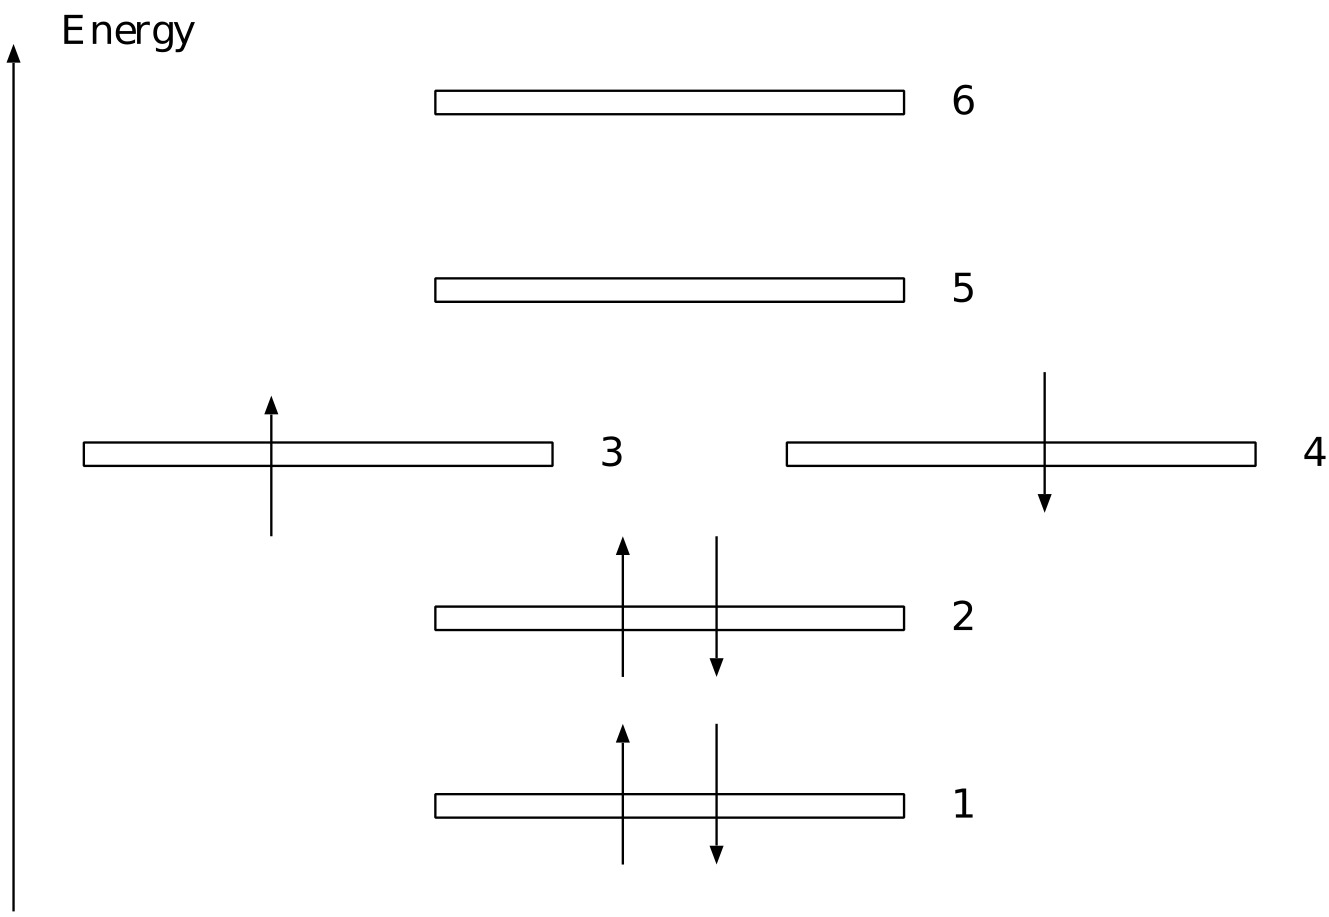
\includegraphics[width=60mm]{figures/CAS1}}
	\subfloat[Slater determinant $|1\bar{1}2\bar{2}3\bar{3}\rangle$]{\label{figure:2}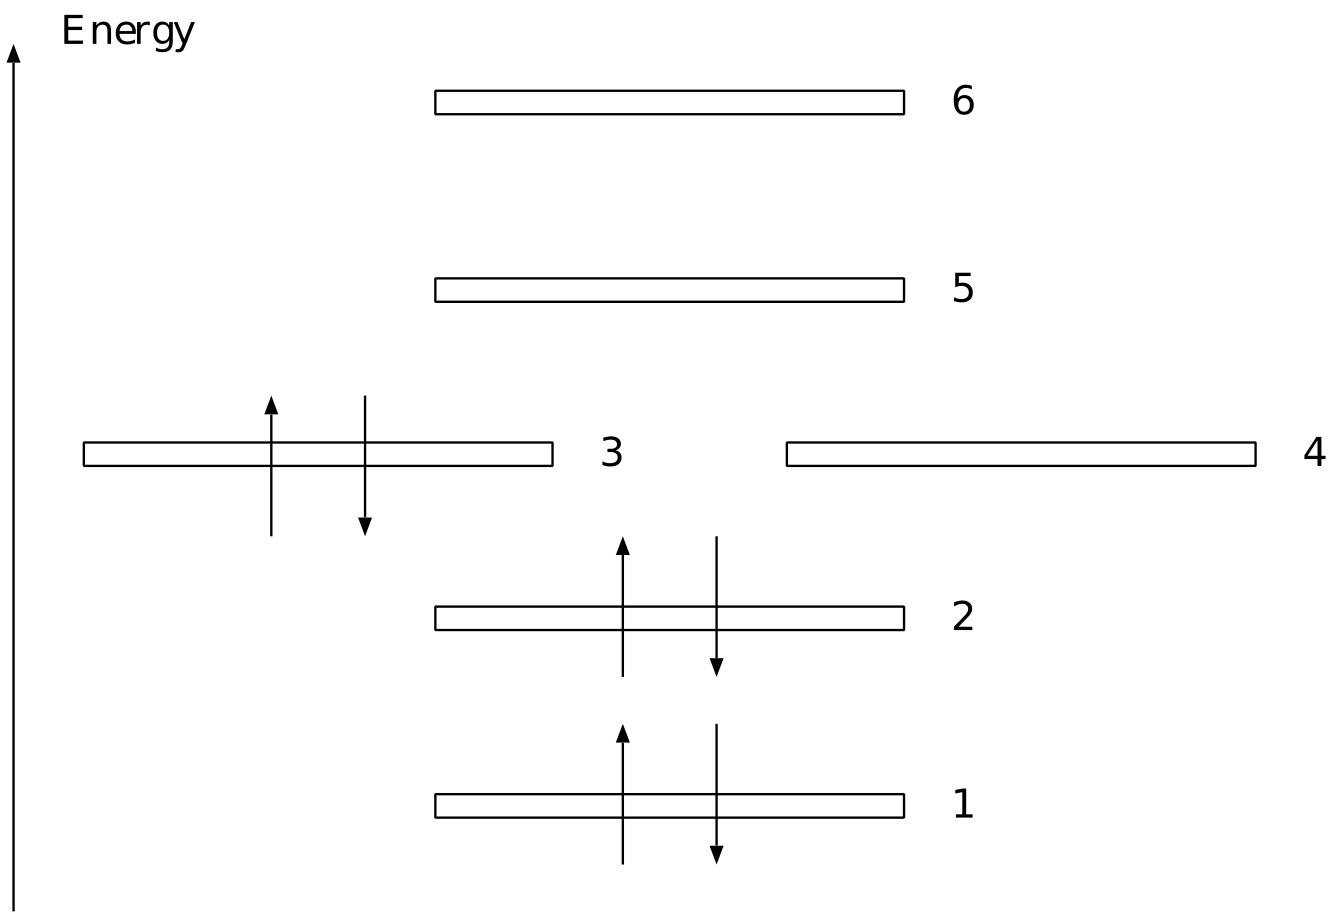
\includegraphics[width=60mm]{figures/CAS2}}
	\\
	\subfloat[Slater determinant $|1\bar{1}2\bar{2}\bar{3}4\rangle$]{\label{figure:3}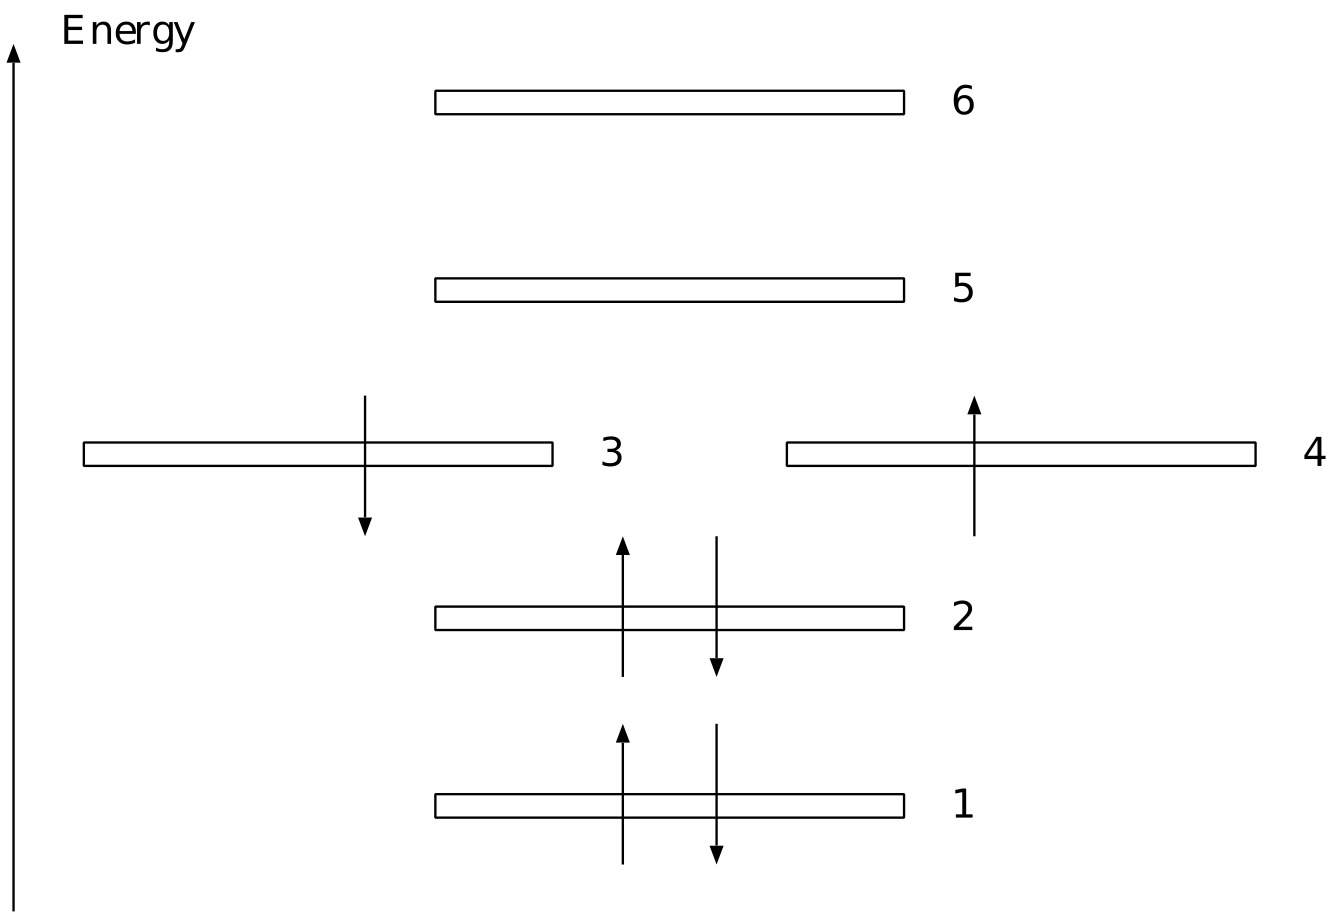
\includegraphics[width=60mm]{figures/CAS3}}
	\subfloat[Slater determinant $|1\bar{1}2\bar{2}4\bar{4}\rangle$]{\label{figure:4}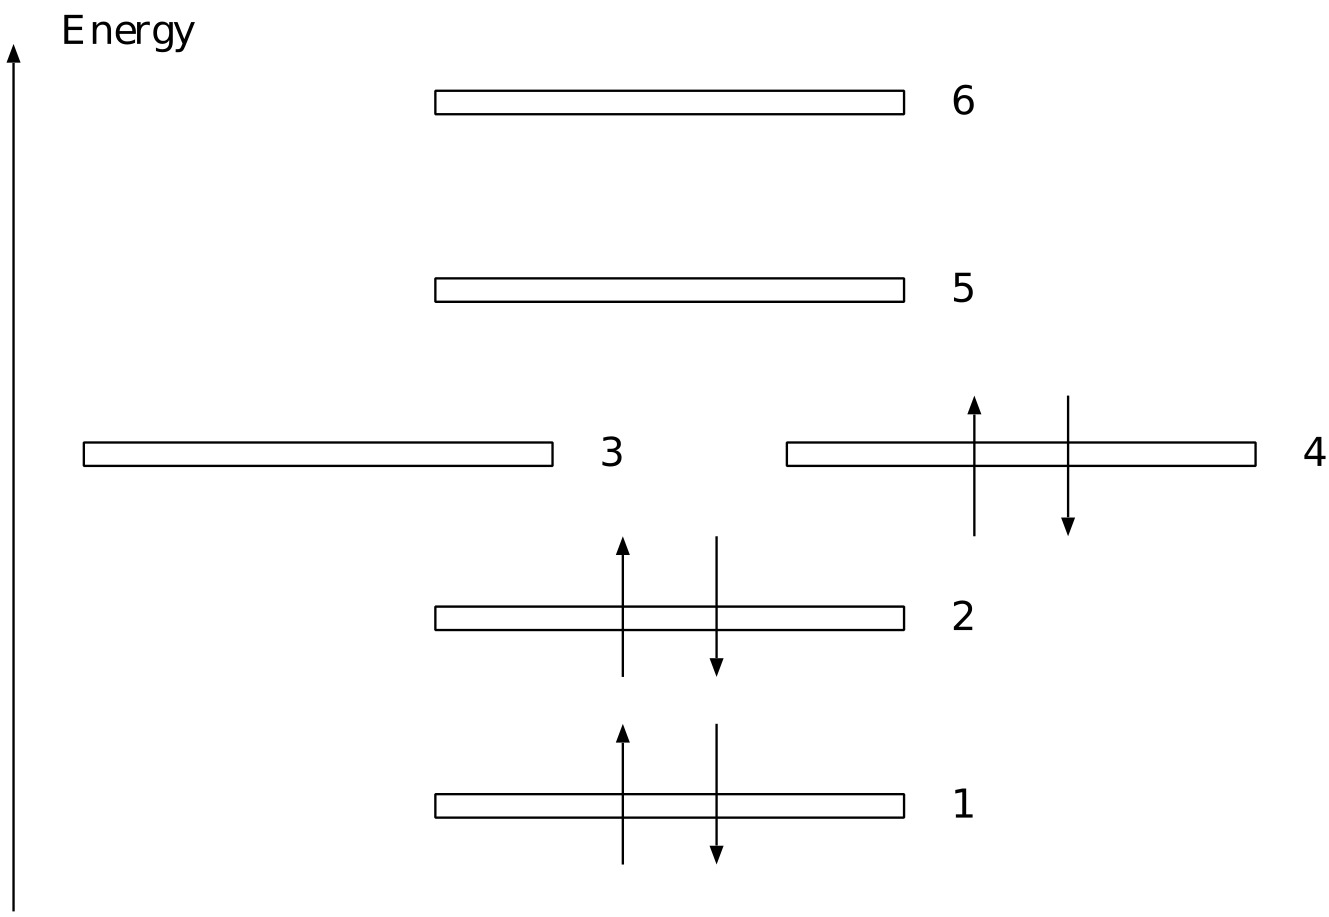
\includegraphics[width=60mm]{figures/CAS4}}
	\label{fig:CAS}
\end{figure}

\begin{figure}
	\centering
	\label{figure}
	\caption{Ground state from figure (1) + single excitation examples (many more exist; number of configurations scale exponentionally with electron population N)}
	\subfloat[Slater determinant $|1\bar{1}2\bar{2}3\bar{5}\rangle$]{\label{figure:5}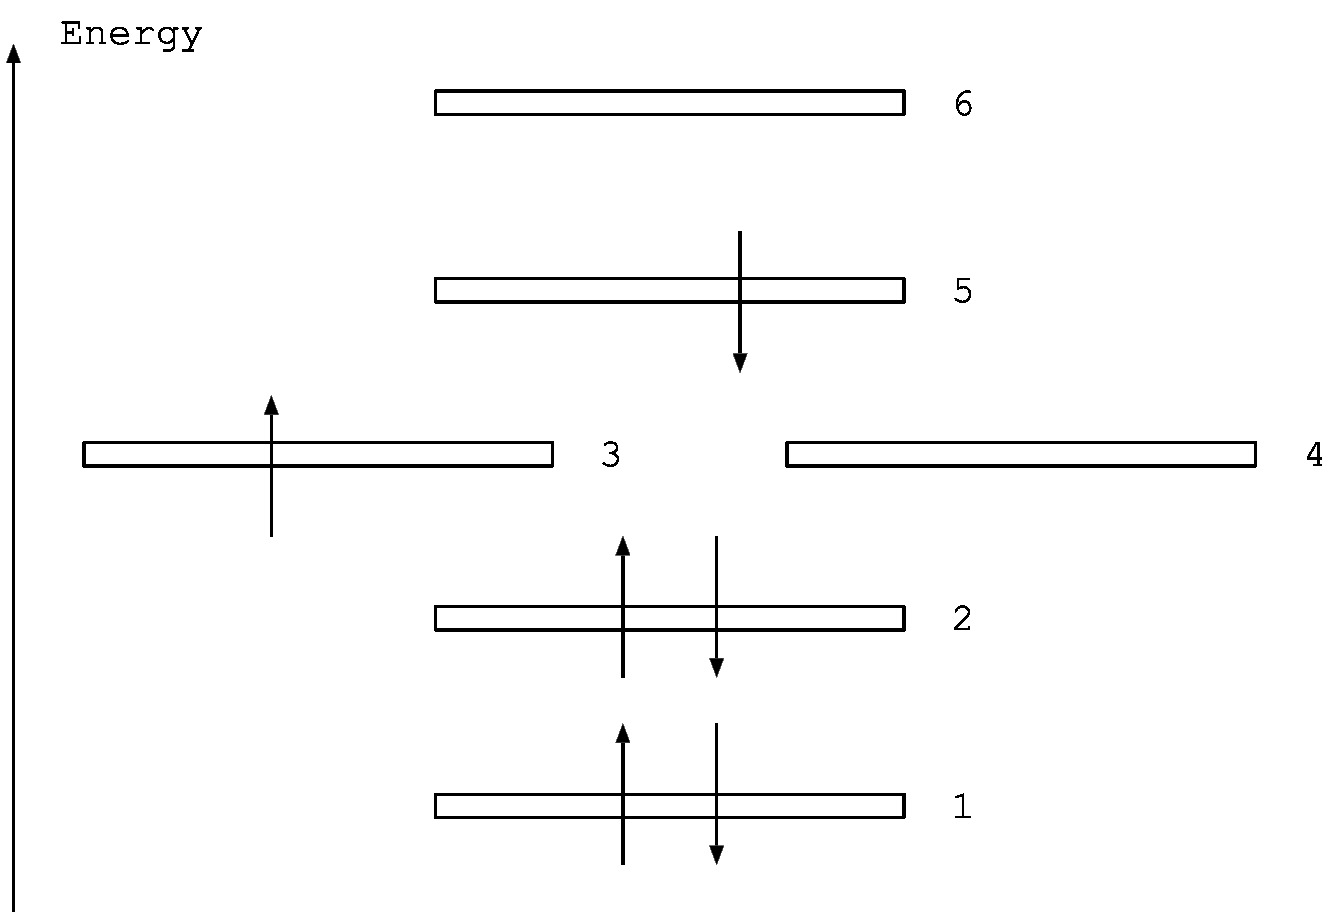
\includegraphics[width=60mm]{figures/CAS+S1}}
	\subfloat[Slater determinant $|1\bar{1}2\bar{2}\bar{4}6\rangle$]{\label{figure:6}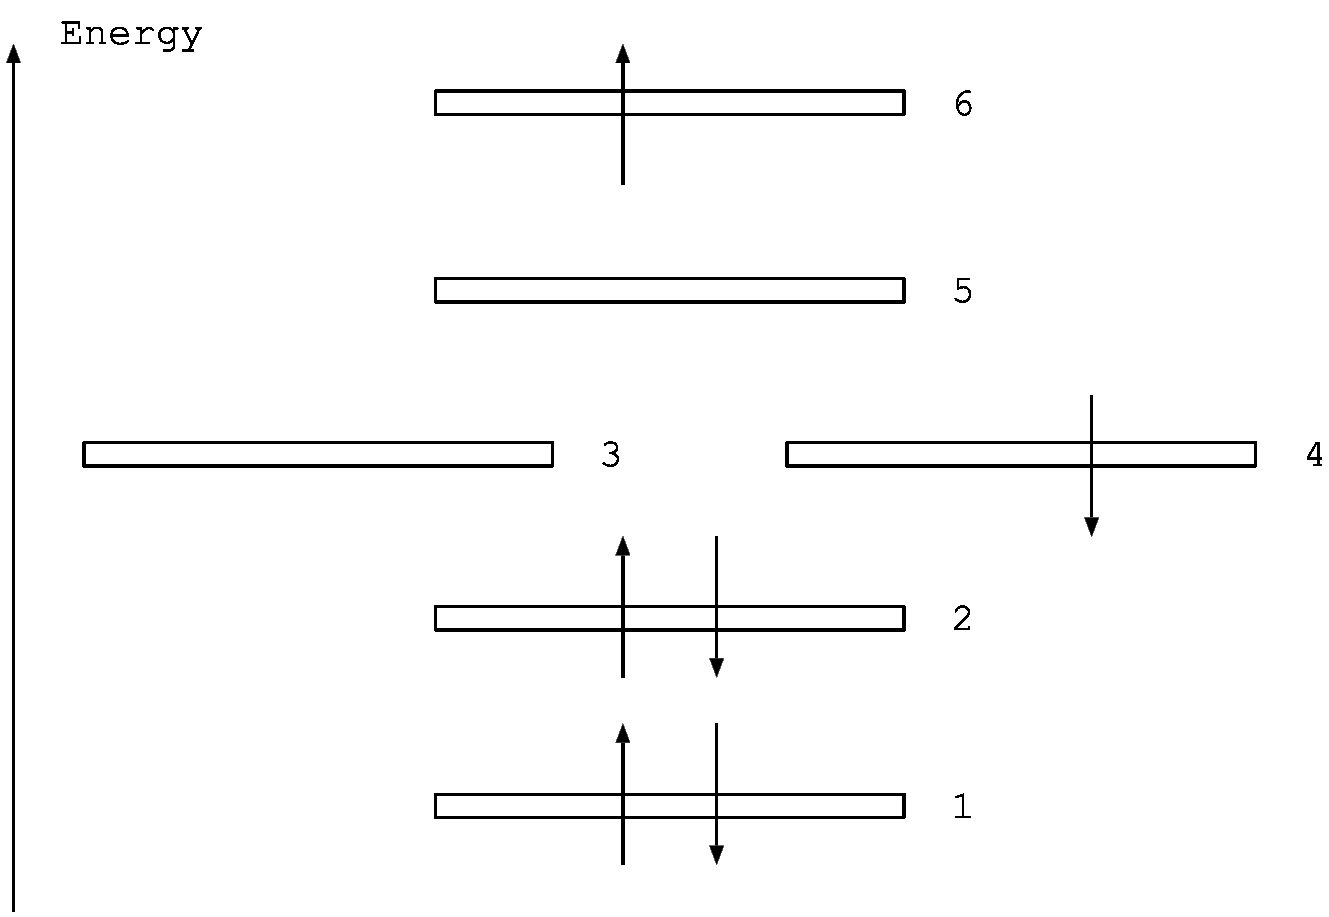
\includegraphics[width=60mm]{figures/CAS+S2}}
	\\
	\subfloat[Slater determinant $|1\bar{1}\bar{2}3\bar{4}5\rangle$]{\label{figure:7}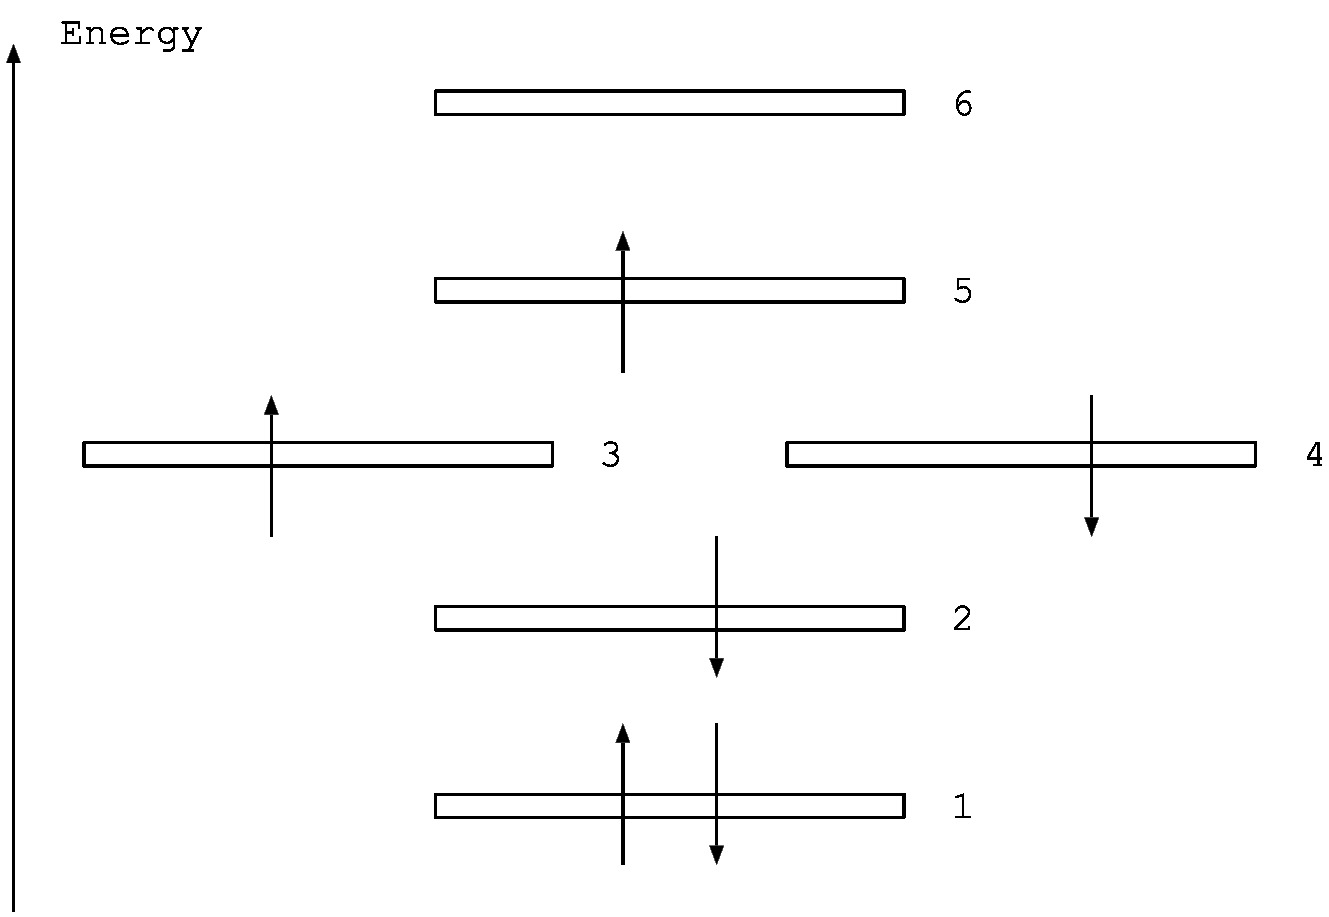
\includegraphics[width=60mm]{figures/CAS+S3}}
	\subfloat[Slater determinant $|12\bar{2}3\bar{4}\bar{6}\rangle$]{\label{figure:8}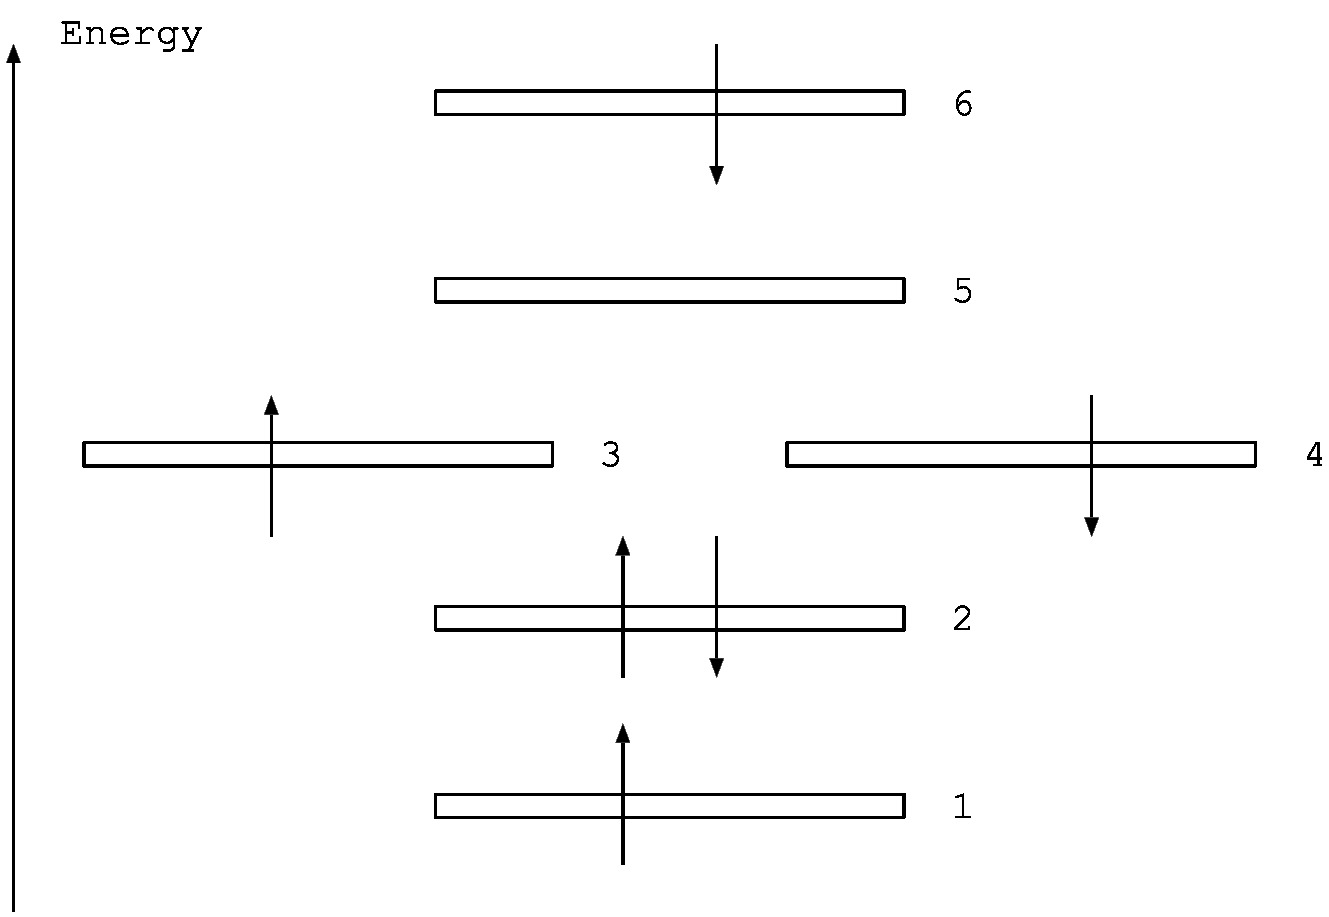
\includegraphics[width=60mm]{figures/CAS+S4}}
\end{figure}
In general, these extended models are very effective at accurately approximating these energies, but some discrepancies appear. An example is the CC3 cluster method which generates excellent agreement with FCI results when the excited states are dominated by a single excitation, but displays considerable error when faced with a large double-excitation character. Another example is the multi-reference method CASPT2, which gives very good results for a large number of systems, but significant errors appear when the reference and outer space are not sharply separated.

DDCI solves these problems by building a configuration interaction with a small reference space, in the subspace of singles and doubles which contributes to the energy difference on the grounds of second-order perturbation considerations, i.e. a subspace defined by the `complete active space' (CAS) for all singles, and the doubles which involved at least one active orbital \cite{garcia1997application}. If faced with a system with numerous open-shells per atom (e.g high-spin manganese, cobalt, iron oxides), the computational cost of using CAS+DDCI or the LCAS+S (`large complete active space + single excitation' method) becomes prohibitive since the size of the space to diagonalise scales exponentially with the number of magnetic electrons. We can establish a simple physical criterion to select important reference configurations, and derive from it a novel method with a strongly reduced computational cost. This is because configurations involved LCAS+S for example, are far too numerous compared to the necessary methods for a good quality modelling of low-lying energy state physics. Something needs to change when approaching this type of problem.

\subsection{Modifications of the Standard WCMs and Effective Hamiltonian Criteria}

Compared to the LCAS+S, the multiple metal-to-metal and ligand-to-metal charge transfer configurations were removed from the reference part of the wavefunction (a ligand is a core electron; the charges being transferred are electrons between ions). When comparing to the CAS+DDCI, the multiple metal-to-metal charge transfer configurations and associated screening configurations were removed. Additionally, double excitations were restricted to screening excitations on the ligand-to-metal charge transfers. This meant that the number of configurations in a magnetic interaction between two high-spin Mn III ions, for CAS+DDCI and LCAS+S, were reduced from approximately 10 billion and 60 billion, to 20 million, respectively. This new approach is called the `selected active space' method (SAS+S); see \cite{gelle2009accurate} for more on this approach. This optimised, embedded fragment, quantum chemical {\it ab initio} method allows for analysis of the local fluctuations of magnetic couplings in manganites, which were known to be influential in the macroscopic magneto-resistance effects but not accessible experimentally.

%%%%%%% Here is wherre my understanding starts to become less than 100%

With both methods a dynamical correlation correction on each reference determinant is included, independent of whether they are based on either the CAS or a zeroth-order multi-reference space retaining the dominant configurations for low-lying states. Highly accurate spectra are consequently obtained, from which effective-exchange integrals can be extracted using an effective Hamiltonian method. This is a Hamiltonian that acts in a reduced space and only describes a part of the eigenvalue spectrum of the true Hamiltonian. The Heisenberg Hamiltonian of equation (1) works on fictitious electron spin variables of magnetic subsystems, describing only low-lying energy states. However, these evaluations yield energy values within the error bar of experimental inelastic neutron scattering results.

The ground and low-lying energy state eigenvalues and wavefunctions provided by these calculations are for a set of fragments designed to suit all the crystallographically independent effective interactions. One can use the described effective Hamiltonian theory to obtain a spin Hamiltonian separate from the Heisenberg one, that also works on fictitious effective electron variables but also nuclear spin variables. It typically only describes the $(2s+1)(2l+1)$ magnetic sublevels of the complete spectrum, where s and l are the spin and orbital angular momentum quantum numbers, respectively. \cite{mostafanejad2014basics}. The objective for the solutions of this spin Hamiltonian is that on each fragment it mimics the eigenvalues of the system that the fragment is embedded within, and that it's eigenvectors reproduce the main configurations of the ab-initio wavefunctions. The projection must be onto a subset of the zeroth-order multi-reference space chosen for the ab-initio calculation, as seen in this equation for the system wavefunction\cite{gelle2009accurate}:

\begin{equation*}
	|\psi_m\rangle = |\psi^0_m\rangle + |\psi^{ct}_m\rangle + |\psi^*_m\rangle
\end{equation*}

where $|\psi^0_m\rangle = \sum_{I}C^0_{I,m}|\Phi^0_I\rangle$, and $|\Phi^0_I\rangle$ represents the zeroth order CAS reference configuration. The coefficients for each determinant are found by diagonalising the effective Hamiltonian. This projection must represent at least $\sim90\%$ of the wave function of all involved states. Once the projection operator that accommodates these requirements is chosen, it is possible to achieve this in minimising the Lagrangian with respect to the fictional effective Hamiltonian variables:

\begin{equation*}
	\min_{J_{ij}} \mathcal{L}(J_{ij}) = \min_{J_{ij}} \sum_I ||\hat{H}(J_{ij})\hat{P}|\Psi_I\rangle-E_I\hat{P}|\Psi_I\rangle||^2
\end{equation*}

$\hat{H}(J_{ij})$ is the spin Hamiltonian, $|\Psi_I\rangle$ is the wave function for the $I$th excited state and $E_I$ its energy, and $\hat{P}$ is the aforementioned projection operator. The accuracy of this chosen $\hat{H}(J_{ij})$ is insured by the fact that $\sqrt{\mathcal{L}(J_{ij})} << J_{ij}$ and about $90\%$ of the \textit{ab initio} wavefunctions are represented for all fragments. 

\section{Calculation of the Displacement with Crystal}
Crystal performs ab initio calculations of the ground state energy as well as the energy gradient. It also has the potential do generate the electron wavefunctions and consequently their behaviour in a periodic system. Hartree-Fock and Kohn-Sham Hamiltonians are typically used (using postulates of DFT). Periodic systems are approximated by expansion of the single-particle wavefunctions as a linear combination of Bloch functions; a wave function that can be written as a plane wave modulated by a periodic function is a Bloch wave, typically used to describe crystallographic electrons. These Bloch functions are modulated by local functions or `Atomic Orbitals'. These are linear `Gaussian type functions' used in the `Linear Combination of Atomic Orbitals' (LCAO) method, which you may know as an approximation that generates a system wavefunction from superposed electronic wavefunctions belonging to individual atoms. The various molecular symmetries (s,p,d,f,sp e.t.c) of the structure are used to modulate these LCAO orbitals \cite{dovesi2017crystal17}.

From a DFT calculation with Crystal, when the optimal geometry is obtained, print the Hessian matrix to file with the option \verb|PRINTHESS|. 


\subsection{Calculation of the J}

From a set of inputs for the software suite used for a point of the calculation
\begin{itemize}
	\item env15
	\item seward
	\item rasscf
	\item localisation
	\item matrec
	\item kinorb
	\item rasscf - ci only
	\item motra
	\item sass
	\item prop
\end{itemize}

\section{Env2Seward}
Env2Seward is a driver script that written in the earlier stages of my time at ILL, to process the output files from the ENV15 program, \texttt{prefix.env.sew0} and \texttt{prefix.env.psd}, that contain the fragment, TIP and Madelung potential coordinates and basis sets (see \cite{varignon2013ab} as well as \cite{gelle2008fast} and the associated local tools manual). It operates by parsing the input files for the various atom types and ordering the data into categorised sets with homogeneous atoms and their associated basis sets from either a default path or chosen library file. They are organised into quantum fragment, pseudopotential and Madelung potential sections in a way that is readable by the SEWARD input algorithm. It can be automated by calling it from command line with a separate shell script, with the libraries and basis sets as a third system input file. 

\section{Solving the displacement equation}
\subsection{Parsing the Born and Hessian files}

Once we have optimised the geometry of a system in order to minimise the total energy i.e. finding the Hessian or minimum critical point of the $3N$ dimensional vector space, where $N$ is the number of atoms in the unit cell, we can generate the output files to be processed in order to solve the displacement of each atom for a given homogenoeous electric field.
The Born tensor is stored in an output file, each $3\times3$ charge matrix categorised under a number of atoms given by a line specifying the population in the unit cell. Once this is found, we can parse for the charge matrices and diagonalise them into a matrix of dimension $3N\times3N$, where the positions are given in terms of Cartesian coordinates. The same goes for the symmetric Hessian, which needs to be parsed from a separate raw output file and arranged into a diagonally symmetric matrix with 3N diagonal elements.

\subsection{Solving for the atom displacements}
Once these tensors have been obtained and reformatted into square form, we can solve the linear equation $q.E = -H.d$ using a linear algebra package. Two possible options would be the more simplistic `numpy linalg' module with the `solve' function, that can solve linear equations of the form $\mathbf{Ax} = \mathbf{b}$, or the LAPACK Fortran drivers that are higher accuracy and specify to the type of matrix you are trying to process (in this case a symmetric semi-definite Hessian) which can save lots of processing time. When the displacements have been obtained, we can add them to the atom coordinates from the generational env15 program and reformat them with env2seward for different values of the electric field. This will be automated so that we can effectively calculate $\frac{\partial d}{\partial E}$ (recall step 5 of section 3).

\bibliography{reportbib.bib}
\bibliographystyle{plainurl}
\end{document}
